\documentclass[10pt]{beamer}
%Information to be included in the title page:
\title{Numerical Simulation of Compound Flooding using Parametric Rainfall Models}
\author{Chayanon (Namo) Wichitrnithed, Eirik Valseth, Younghun Kang, Mackenzie Hudson, Ethan Kubatko, Clint Dawson}
\institute{UT Austin - Oden Institute for Computational Engineering and Sciences, Ohio State University}
\date{November 2022}

\usetheme{Madrid}
\newcommand\dt[1]{\frac{\partial #1}{\partial t}}
\newcommand\dx[1]{\frac{\partial #1}{\partial x}}
\newcommand\dy[1]{\frac{\partial #1}{\partial y}}

\begin{document}

\frame{\titlepage}

\begin{frame}
\frametitle{Compound Flooding}
This is some text in the first frame. This is some text in the first frame. This is some text in the first frame.
\end{frame}

\begin{frame}
  \frametitle{Computational Difficulties}
\end{frame}

\begin{frame}
  \frametitle{Mathematical Model}
  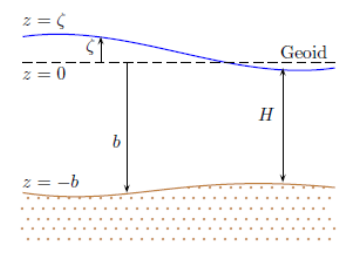
\includegraphics[width=0.5\textwidth]{bathy.png}
\end{frame}

\begin{frame}
  \frametitle{Mathematical Model}
  Assuming depth is small relative to horizontal scale, we can average over the z-direction to obtain
  \begin{block}{The Shallow Water Equations}
    \begin{align*}
      \dt{\zeta} + \dx{(Hu)} + \dy{(Hv)}  &= S(t,x,y) \\
      \dt{(Hu)} + \dx{(Hu^2)} + \dy{(Huv)} &= -gH\dx{\zeta} + F_x \\
      \dt{(Hv)} + \dx{(Huv)} + \dy{(Hv^2)} &= -gH\dy{\zeta} + F_y
    \end{align*}
  \end{block}
  where \\
  $\zeta =$ surface elevation \\
  $H = $ total depth \\
  $u,v = $ depth-averaged horizontal velocities \\
  $F_x,F_y = $ horizontal forces including friction \\
  $S = $ source/sink term
\end{frame}

\begin{frame}
  \frametitle{Compact Form of the Equations}
  Rewriting terms into matrix/vector form  gives
  \begin{block}{The Shallow Water Equations (divergence form)}
    \begin{align*}
    \dt{\mathbf{w}} + \nabla \cdot \mathbf{F}(\mathbf{w}) = \mathbf{r}(\mathbf{w})
    \end{align*}
  \end{block}
  where
  \begin{align*}
    \mathbf{w} &= [\zeta, uH, vH]^T \\
    \mathbf{r} &= [S, gH\dx{\zeta} + F_x, gH\dy{\zeta} + F_y]^T \\
    \mathbf{F} &=
                 \begin{bmatrix}
                   uH & vH \\
                   Hu^2 + g(H^2-h^2) & Huv \\
                   Huv & Hv^2 + g(H^2-h^2)
                 \end{bmatrix}
  \end{align*}
\end{frame}

\begin{frame}
  \frametitle{Computational Method}
  \begin{itemize}
  \item DG-SWEM uses the discontinuous Galerkin (DG) method to discretize in space and Runge-Kutta in time
  \item Combines advantages of FEM and FVM:
    \begin{itemize}
    \item Finite element: high-order basis functions, works well on complex geometries
    \item Finite volume: designed for conservation laws, guarantees local mass conservation, stability achieved from numerical flux
    \end{itemize}
  \end{itemize}
  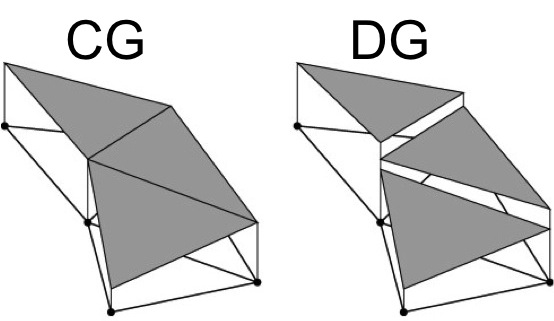
\includegraphics[width=0.5\textwidth]{cgdg.jpg}
\end{frame}
\begin{frame}
  \frametitle{Computational Domain}
  \begin{figure}[t]
    \centering
    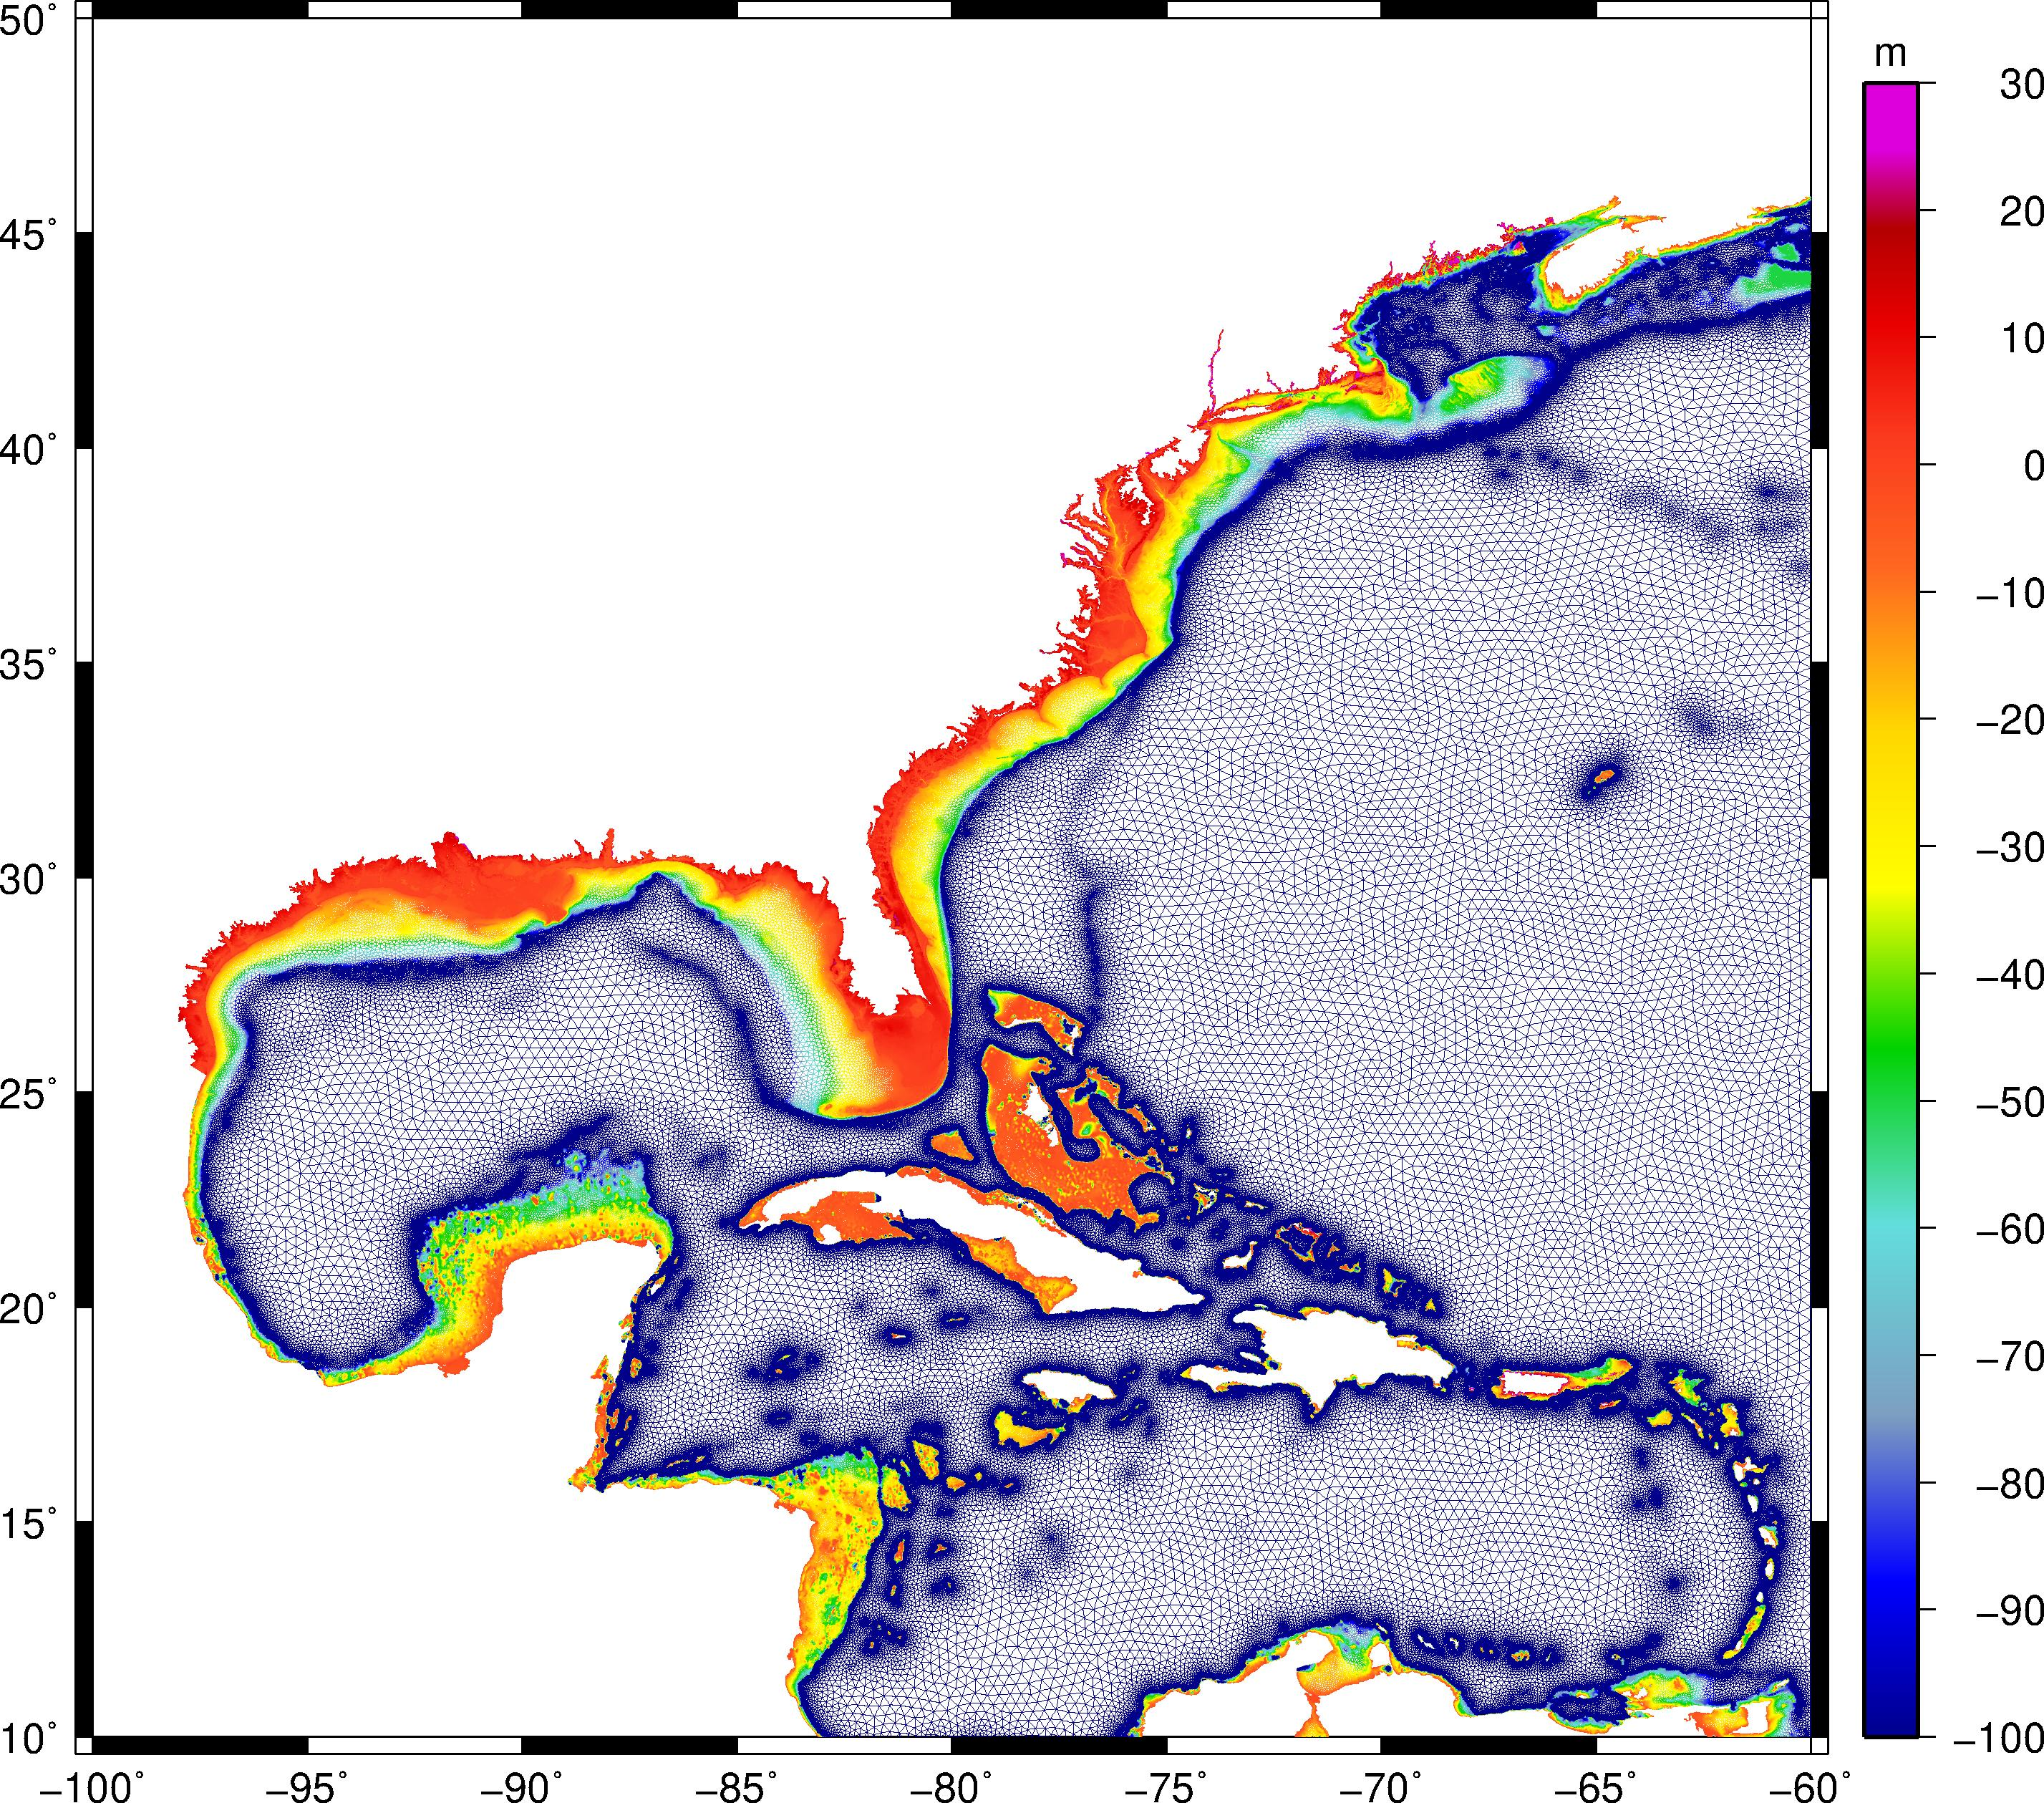
\includegraphics[width=0.7\textwidth]{120m_bath.jpg}
  \end{figure}
\end{frame}

\begin{frame}
  \frametitle{Incorporating rainfall}
  \begin{itemize}
  \item Manually specify rain intensity (m/s) at each node in the grid
    \begin{itemize}
    \item Useful for hindcasting given avaiable rain data
    \item Need to preprocess additional output
    \end{itemize}
  \item Use parametric rainfall models
    \begin{itemize}
    \item Rain intensity at each point can be approximated by storm data
    \item If works, useful for forecasting
    \item Existing parametric models have been studied (see paper)
    \end{itemize}
  \end{itemize}
\end{frame}
\begin{frame}
  \frametitle{Parametric rainfall models}
  \begin{itemize}
  \item R-CLIPER model (Panton, 2002)
  \item IPET model
  \end{itemize}
\end{frame}

\begin{frame}
  \frametitle{Storm data}
\end{frame}

\begin{frame}
  \frametitle{Test case: Hurricane Harvey (2017)}
  \begin{itemize}
  \item A good representative for compound flooding
  \item Total rain: 51 inches in the Houston city area
  \item Surge relatively low
  \item Run on TX 2008 mesh from Aug - Sep 2017
  \item Using 34,000 CPU, took about 12 hours
  \end{itemize}
  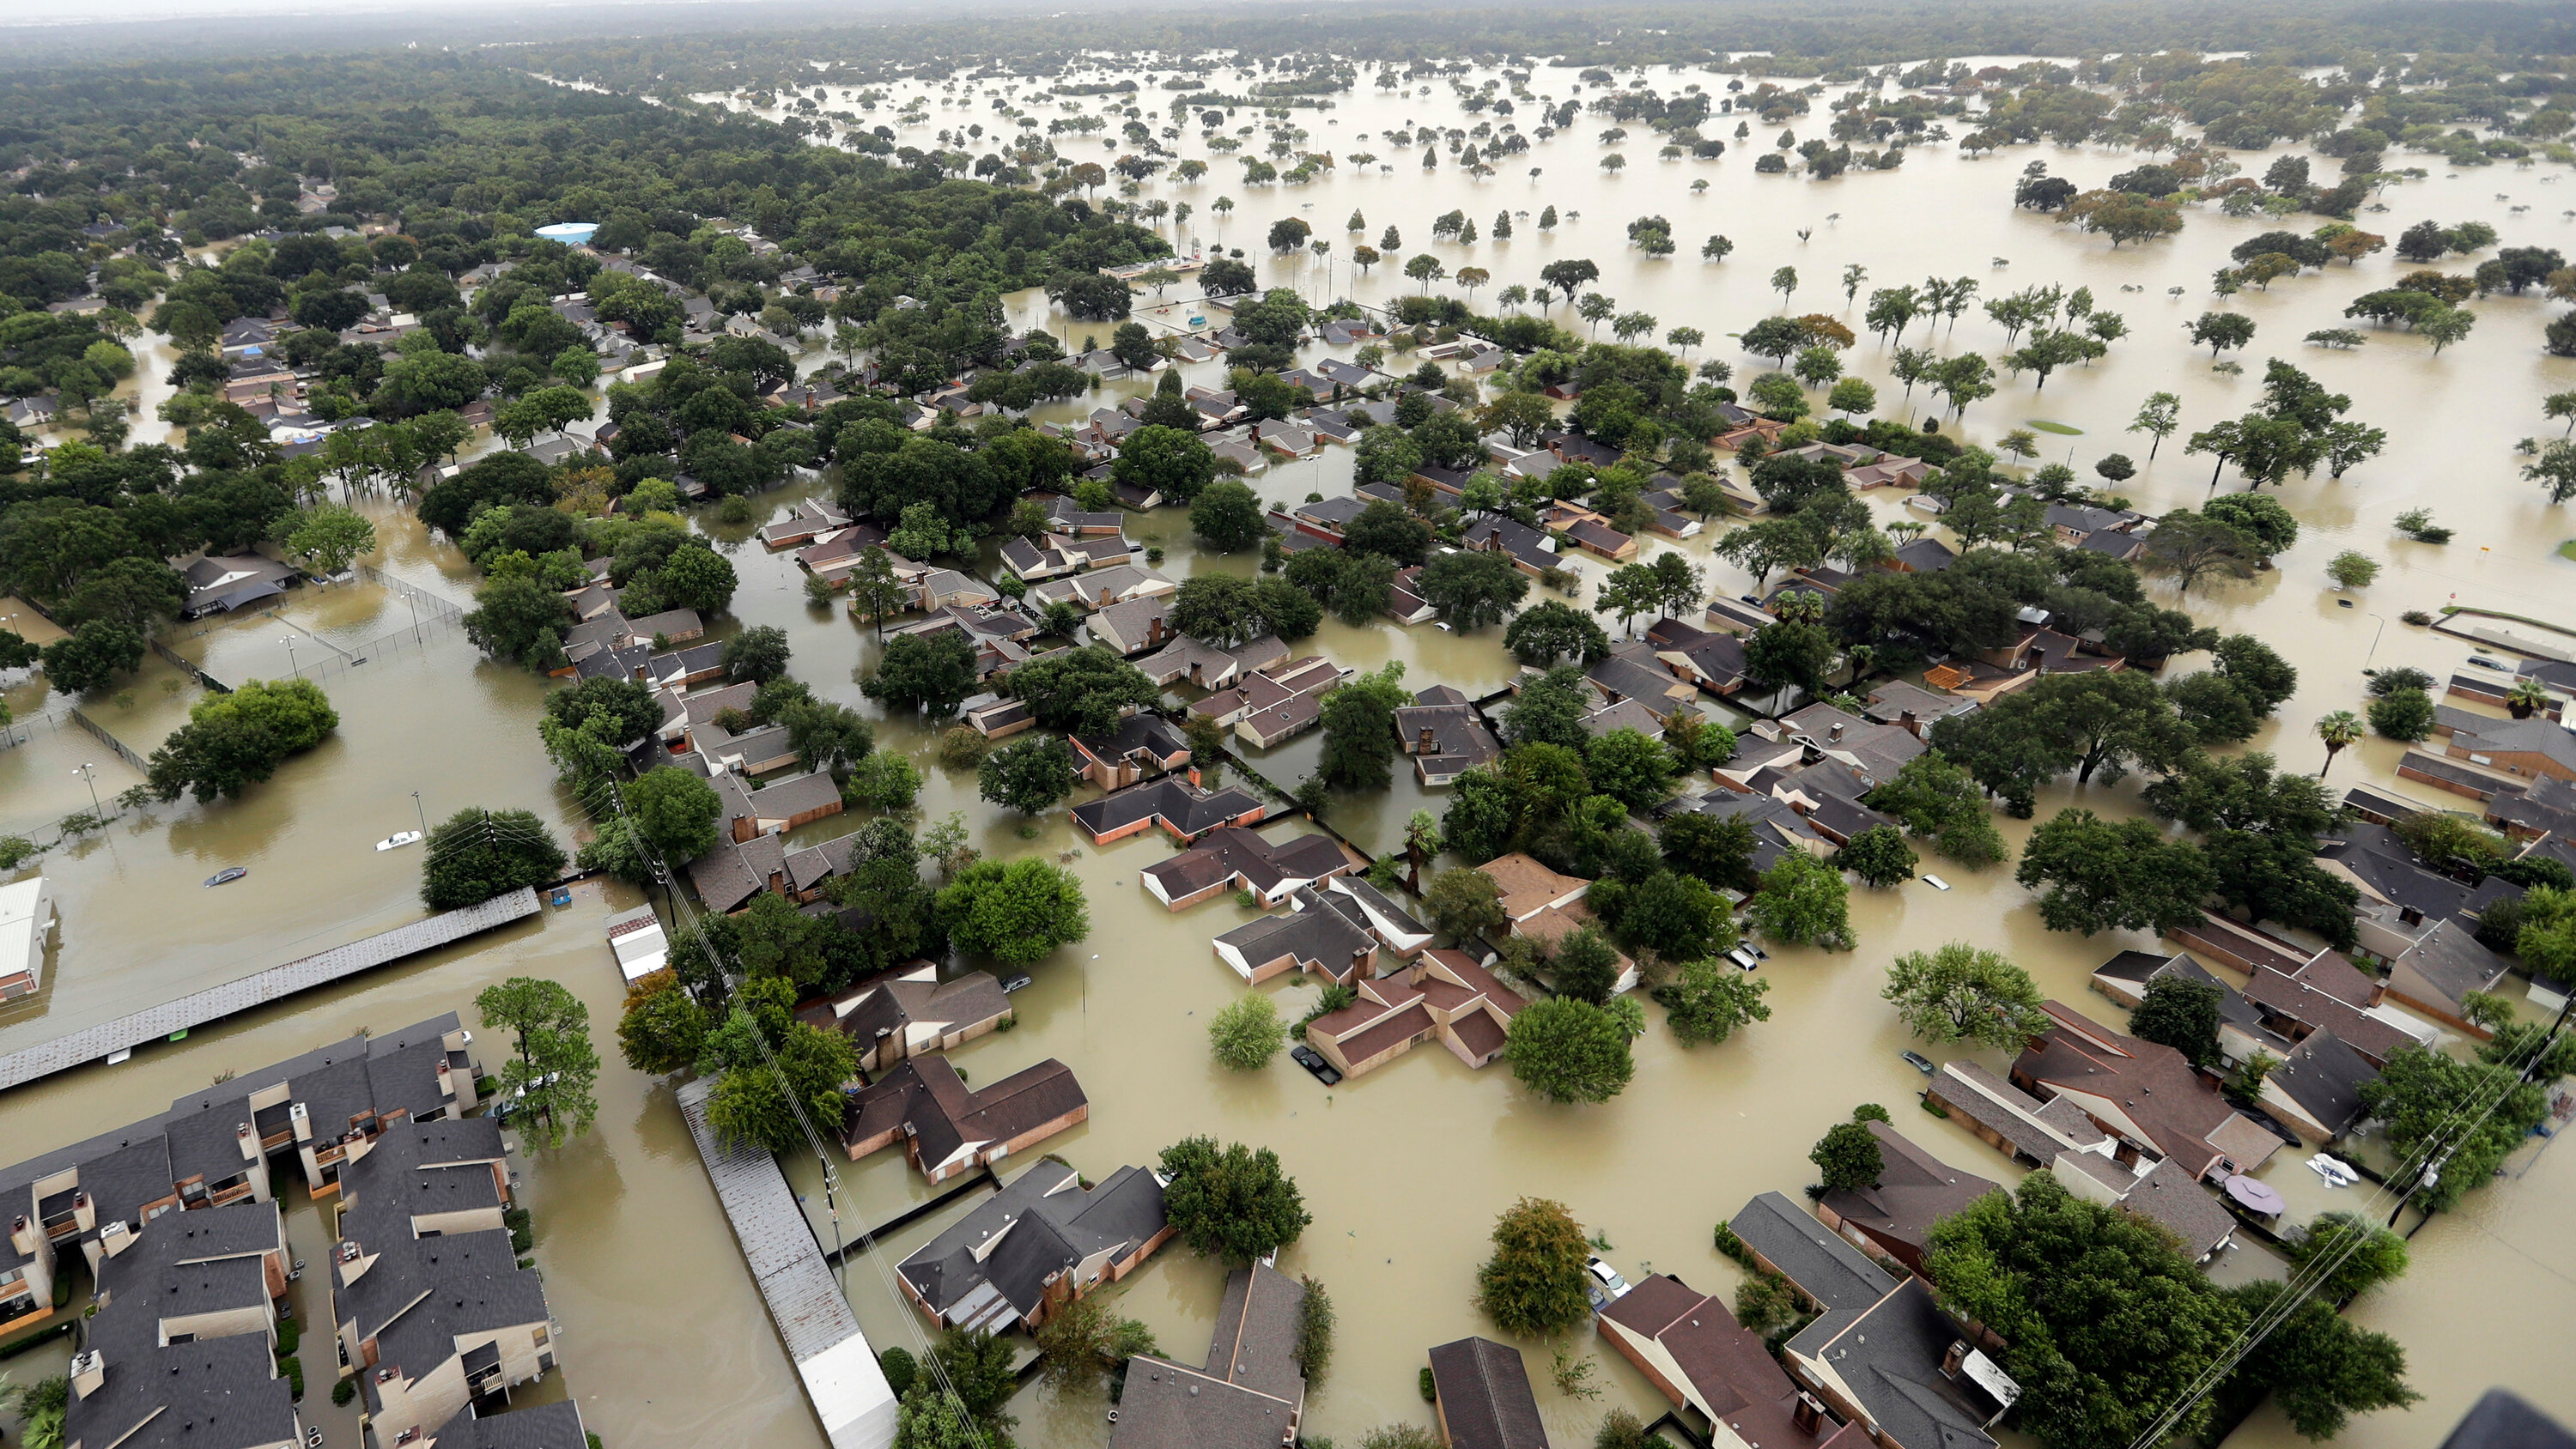
\includegraphics[width=0.7\textwidth]{harvey.jpg}
\end{frame}
\begin{frame}
  \frametitle{Results}
  \begin{itemize}
  \item Hydrographs
  \end{itemize}
\end{frame}

\begin{frame}
  \frametitle{Results (HMW)}
\end{frame}

\end{document}